			\documentclass[10pt,a4paper]{article}
			\usepackage[english]{babel}
			\usepackage[utf8]{inputenc}
			\usepackage{fancyhdr}
			\usepackage{hyperref}
			\usepackage{graphicx}
			\usepackage{subcaption}
			\usepackage{caption}
			\usepackage{cite}
			\usepackage{booktabs}
			\usepackage{wrapfig}
			\usepackage{float}
			\usepackage{amsmath}
			\usepackage{xcolor}
			\usepackage{listings}
			
			\restylefloat{table}
		
			\pagestyle{fancy}
			\fancyhf{}
			\rhead{17-May-2018}
			\lhead{Assignment 04}
			\rfoot{Page \thepage}
		
			\begin{document}
			\begin{titlepage}
			\centering
		
				{\scshape\LARGE Scientific Experimentation and Evaluation\par}
		
				{\scshape\Large Assignment: 04\par}
		
				\vfill
		
				\vfill
				{\Large\itshape Anees Khan (9030423)
					\\Debaraj Barua (9030412)\\
					Md Zahiduzzaman (9030432)
					\par}
				\vfill
		
				{\large 17-May-2018\par}
			\end{titlepage}
			\tableofcontents
			\listoffigures	
			\listoftables
			\newpage
			\section{Relevant Aspects of Experiment}
			\subsection{Design of Robot}
				\begin{itemize}
					\item The robot has been designed with three wheels.
					\item Two of these are driving wheels and are connected to the motors, thus enabling a differential drive systems; and \textcolor{black}{the third is a caster wheel at the back}.
					\item Wheels are oriented as shown in the \textcolor{black}{images below}.
					\begin{figure}[H]
						\begin{subfigure}{0.5\textwidth}
							\centering
							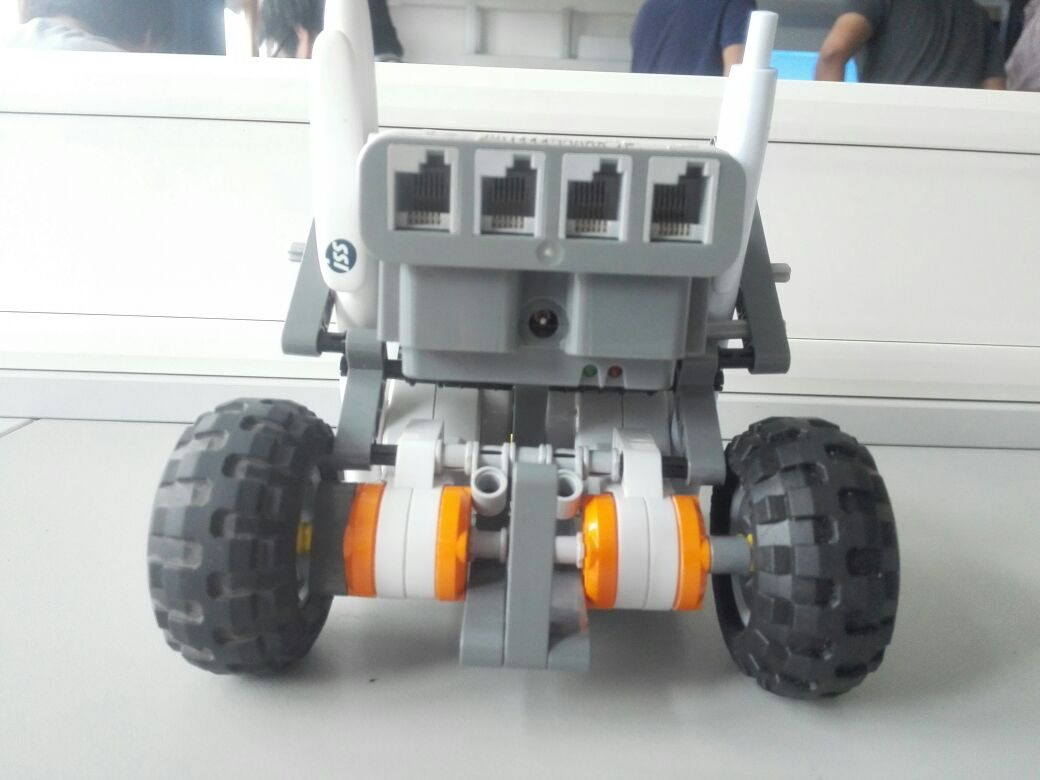
\includegraphics[width=0.8\linewidth]{img/front.jpeg}
							\caption{Front View}
							\label{fig:fview}
						\end{subfigure}%
						\begin{subfigure}{0.5\textwidth}
							\centering
							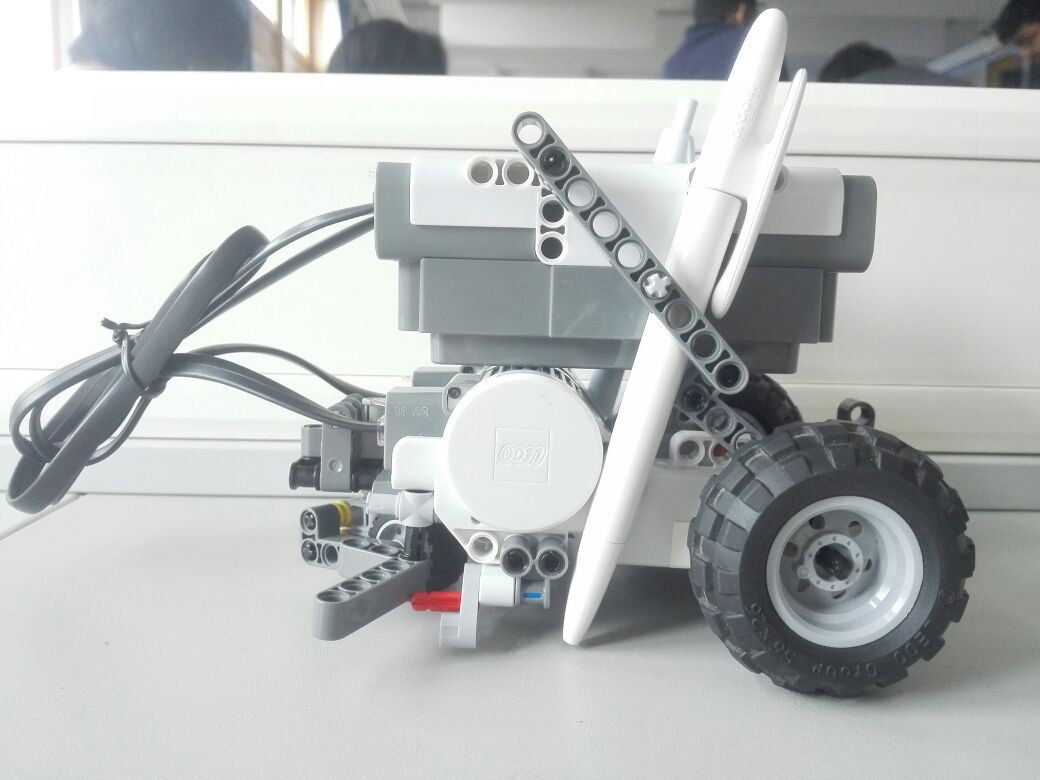
\includegraphics[width=0.8\linewidth]{img/right.jpeg}
							\caption{Right View}
							\label{fig:rview}
						\end{subfigure}
						\begin{subfigure}{0.5\textwidth}
							\centering
							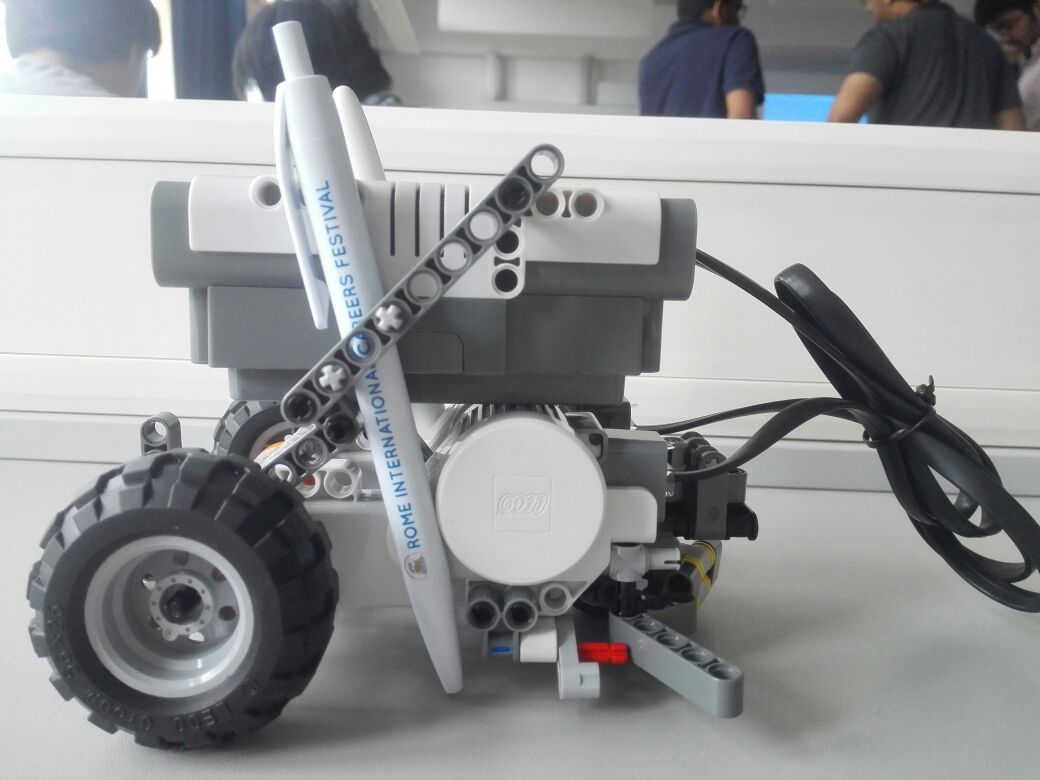
\includegraphics[width=0.8\linewidth]{img/left.jpeg}
							\caption{Left View}
							\label{fig:lview}
						\end{subfigure}
						\begin{subfigure}{0.5\textwidth}
							\centering
							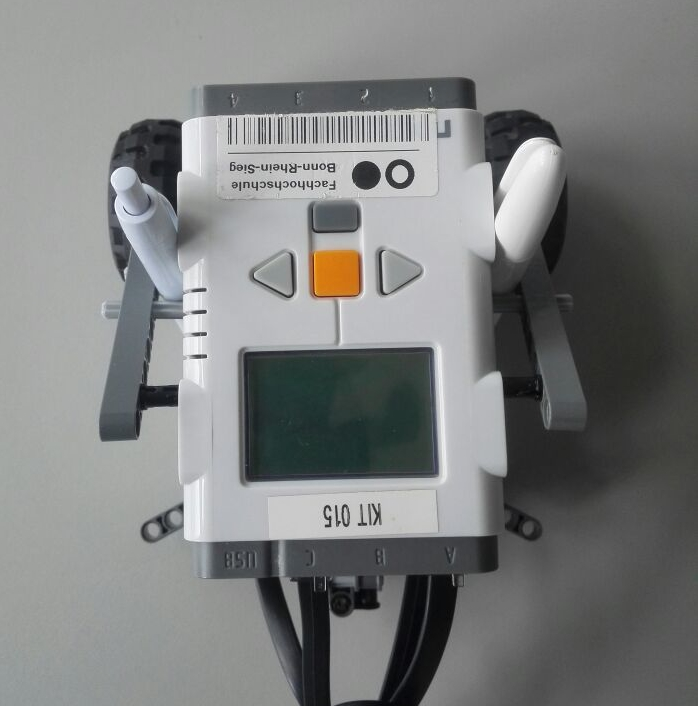
\includegraphics[width=0.8\linewidth]{img/top.jpeg}
							\caption{Top View}
							\label{fig:tview}
						\end{subfigure}
						\begin{subfigure}{0.5\textwidth}
							\centering
							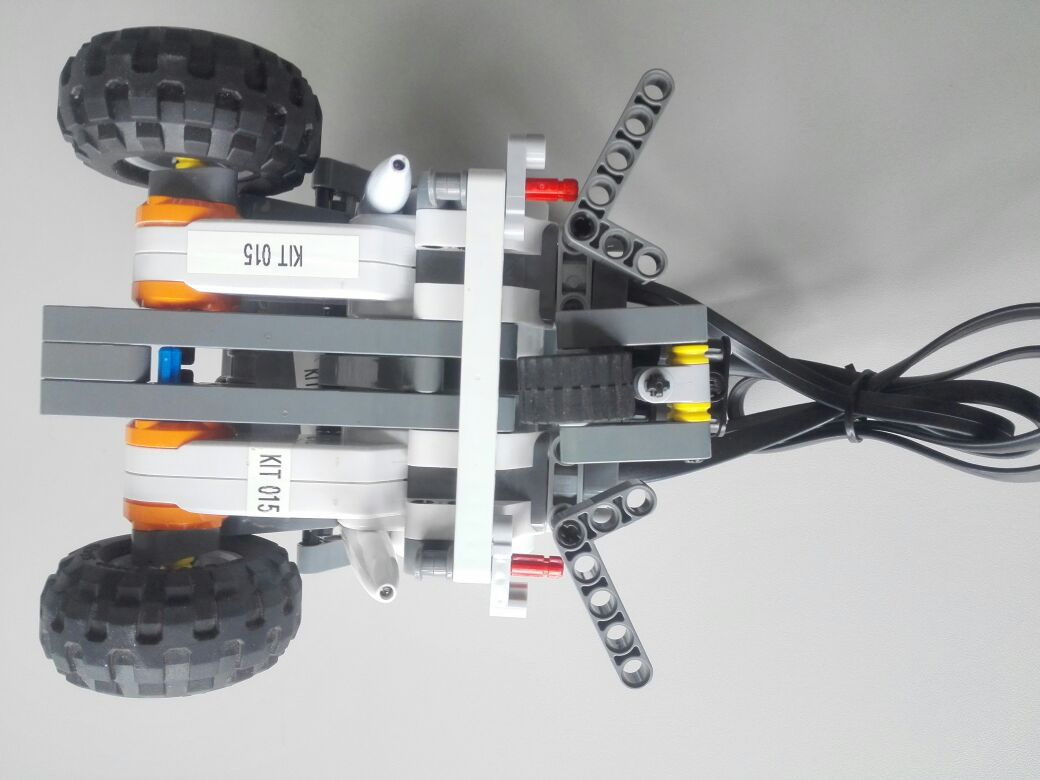
\includegraphics[width=0.8\linewidth]{img/bottom.jpeg}
							\caption{Bottom View}
							\label{fig:bottomview}
						\end{subfigure}
						\caption{Robot Design}
						\label{fig:Robotfig}
					\end{figure}
					\item \textcolor{black}{In addition, it is ensured that the caster wheel cannot rotate completely, and its rotation is limited as shown in the bottom view}.
				\end{itemize}
			\documentclass[paper=a4, fontsize=11pt]{scrartcl} % A4 paper and 11pt font size

\usepackage{amsmath,amsfonts,amsthm} % Math packages


\begin{document}


\section{Ground truth}

\begin{align} 
\begin{split}
R 	&= \frac{l}{2} \frac{V_l + V_r}{V_r - V_l}
\end{split}					
\end{align}

\begin{align} 
\begin{split}
\omega 	&= \frac{V_r - V_l}{l}
\end{split}					
\end{align}

\begin{align} 
\begin{split}
ICC 	&= [x - R sin(\theta), y + R cos(\theta)]
\end{split}					
\end{align}


\begin{align}
\begin{bmatrix}
x^{'} \\
y^{'} \\
\theta^{'}
\end{bmatrix}
= 
\begin{bmatrix}
cos(\omega \delta t) & -sin(\omega \delta t) & 0\\
sin(\omega \delta t) & -cos(\omega \delta t) & 0\\
0 & 0 & 1
\end{bmatrix}
\begin{bmatrix}
x - ICC_x\\
y - ICC_y \\
\theta
\end{bmatrix}
+
\begin{bmatrix}
ICC_x\\
ICC_y \\
\omega \delta t
\end{bmatrix}
\end{align}

Where,
\begin{itemize}
	\item $l$ is the distance between the centers of the two wheels
	\item $Vr, Vl$ are the right and left wheel velocities along the ground
	\item $R$ is the signed distance from the Instantaneous Center of Curvature (ICC) to the midpoint between the wheels
	\item $\omega$ is the rate of rotation about the ICC
\end{itemize}



\end{document}
			\subsection{\textcolor{black}{Transformations}}							
				\begin{itemize}
					\item Perpendicular distance from pen axis to wheel axis = 4.6 cm
					\item Distance between the mid points of the two wheels (track width) = 11.1 cm
					\item The axis of the wheel is considered to be parallel to the axis formed by joining the two pens.
					\item 	To calculate the center of motion for robot, we use the function as shown below.
					\item The \textit{row} variable has three components, $x$ and $y$ coordinates of the center between two pens and the orientation angle of the robot. 
				\end{itemize}
\begin{lstlisting}[language=Python]
def computeCenterOfMotion(data):
	com = np.zeros((data.shape[0],3))
	for i,row in enumerate(data[:]):
		x = row[0]+distance_between_axes*np.cos(np.deg2rad(row[2]))
		y = row[1]+distance_between_axes*np.sin(np.deg2rad(row[2]))
		com[i,:]=np.array([x,y,row[2]])        
	return com
\end{lstlisting}
			
			\subsection{Measurement of Start and Stop Positions}
				\subsubsection{\textcolor{blue}{Measurement Instruments}}
					\begin{itemize}
						\item Distance:
						\begin{itemize}
							\item We use a scale ruler to measure the distances.
							\item In addition, we also utilize the grids on the paper which acts as our workspace and world coordinate systems.
							\item Instrument Details:
							\begin{itemize}
								\item 1 square of the grid paper equals $2.5 \times 2.5$ cm
								\item The precision of the scale used is 1 mm.
							\end{itemize}
						\end{itemize}
						\item Angle:
						\begin{itemize}
							\item A protractor is used as a measuring instrument for the angles.
							\item Instrument Details:
							\begin{itemize}
								\item Precision of the protractor used is 1$^\circ$.
							\end{itemize}
						\end{itemize}
					\end{itemize}
				\subsubsection{\textcolor{black}{Measurement Procedure}}
				\begin{itemize}
					\item Two pens will be fixed near the two driving wheels.
					\item The starting position is where the two pens meets the x -axis, with the left pen lying on the origin (right pen at a distance of  8.3 cm from the origin).			
					\begin{figure}[h]
						\centering
						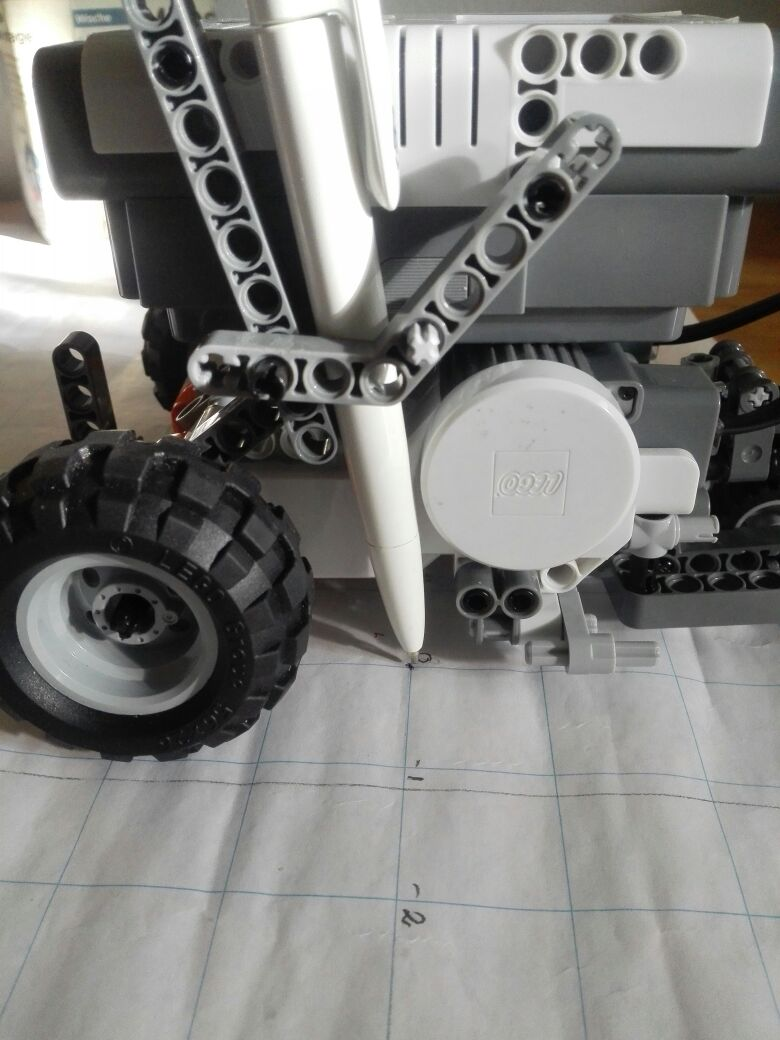
\includegraphics[width=0.4\linewidth]{img/starting-pt.jpeg}
						\caption{Staring Position}
						\label{fig:startingView}
					\end{figure}
					\item To measure the orientation of robot, the two points from these pens will be joined by drawing a line, which will be used to mark the pose of robot, with respect to the coordinate system defined.
					\item For each run, at the initial condition, it is ensured that orientation of rear caster wheel axle is parallel to the driving wheel axis.
					\item Measuring Position:
						\begin{itemize}
							\item To get the position of the robot, we measure the distance of the two points from X and Y axis using a scale ruler.
							\item These two readings are put in the transformation equation described above to get the actual position of the robot.
						\end{itemize}
					\item Measuring Angles:
						\begin{itemize}
							\item The angular pose of the robot is the angle the X-axis makes with the normal to the line joining the two points.
							\item This angle is equal to the angle Y-axis makes with the line joining the two points. This can be verified using basic geometry, as shown in the image below.
							\begin{figure}[h]
								\centering
								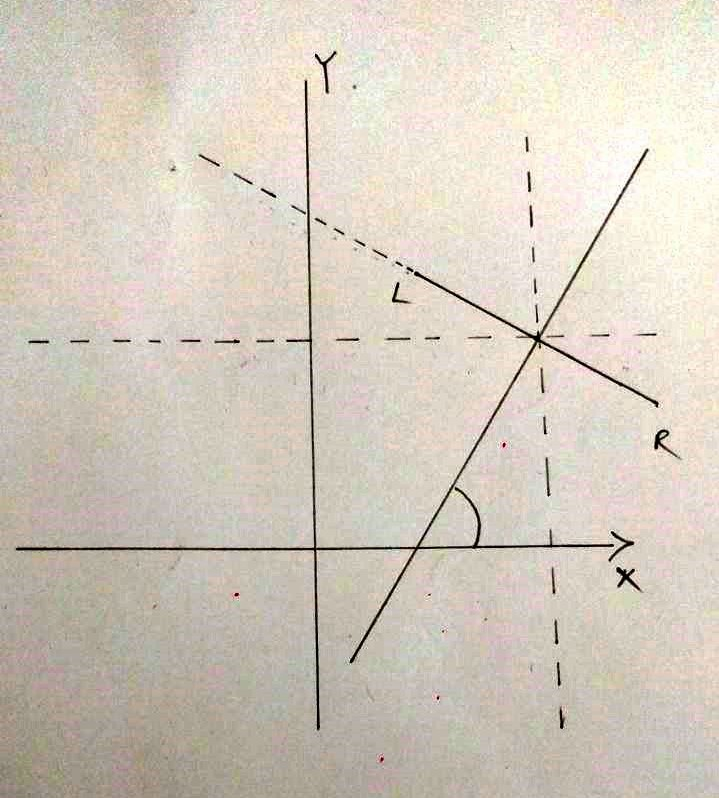
\includegraphics[width=0.4\linewidth]{img/angles.jpeg}
								\caption{Measurement of angles}
								\label{fig:angGeometry}
							\end{figure}
							\item We now measure the angle using a protractor.
						\end{itemize}
				\end{itemize}
			\subsection{Parameters used to drive the robot}
				\begin{itemize}
					\item Constant angular and translational speed for a fixed time period to describe an arc to left.
					\item Constant translational speed and no angular speed for a fixed time period to describe a straight line.
					\item Constant angular and translational speed for a fixed time period to describe an arc to right.
					\item Speed = 18 cm/s
					\item Duration = 2.25 seconds
					\item Turn Rate = 40
					\item Diameter of wheels: 5.7 cm
				\end{itemize}
			\subsection{Program used to drive the robot}
				\begin{itemize}
					\item Using the JAVA code shared in LEA, we created the scenarios for three run sequences.
					\item Straight Line:
						\begin{itemize}
							\item Speed = 18 cm/s
							\item Duration: 2.25 Seconds
							\item Turn Rate = 0
						\end{itemize}
					\item Left Arc:
						\begin{itemize}
							\item Speed = 18 cm/s
							\item Duration: 2.25 Seconds
							\item Turn Rate = 40
						\end{itemize}
					\item Right Arc:
						\begin{itemize}
							\item Speed = 18 cm/s
							\item Duration: 2.25 Seconds
							\item Turn Rate = -40
						\end{itemize}							
				\end{itemize}
			\subsection{Expected Problems and Performance}
				\begin{itemize}
					\item Axis connecting the two pens might not be parallel to the wheel axle.
					\item Start position of each run may not be exactly similar owing to inaccurate positioning of the robot, this will result in lower precision.
					\item Pens may slip of move during the run, as such may not result in accurate positions, thus affecting the precision of our readings.
					\item The constant angular and translational speeds that we assume, may be inaccurate. The actual speed may differ and thus our estimate from the time will be inaccurate.
					\item The initial acceleration and final deceleration of the robot has not been considered in the experiments, resulting in low accuracy.
					\item In addition of the two previous points, slippage in the wheels and motors will also affect the accuracy of readings.
					\item The caster wheel will also result in the bot to drift and also decrease the distance it reaches.
					\item In addition, the calculation of expected position may result in an overestimate because actual power output may depend on the charge in batteries and the efficiency of motor.
				\end{itemize}
			\section{\textcolor{blue}{Observations and Data}}
				\subsection{Readings}
					\begin{table}[H]
						\centering
						\input{initial}
						\caption{Intial Position}
					\end{table}
					\begin{table}[H]
						\centering
						\begin{table}[H]
\centering
\caption{Final Pose along straight direction}
\label{straight}
\begin{tabular}{|l|c|c|c|}
	\hline
	\multicolumn{1}{|c|}{Object Type} & X (cm) & Y (cm) &  $\theta$ (radians)   \\ \hline
	Small                             & -90.34 & -75.31 & 1.40				    \\ %\hline
	Medium                            & -87.85 & -71.63 & 1.48				    \\ %\hline
	Large                             & -84.00 & -67.94 & 1.39    				\\ \hline
	Combined                          & -87.40 & -71.63 & 1.42				    \\ \hline
\end{tabular}
\end{table}

						\caption{Straight Line Position}
					\end{table}
					\begin{table}[H]
						\centering
						\input{leftArc}
						\caption{Left Arc Position}
					\end{table}
					\begin{table}[H]
						\centering
						\input{rightArc}
						\caption{Right Arc Position}
					\end{table}
				 \subsection{Visualization}
					 \begin{figure}[H]
						 	\begin{subfigure}{\textwidth}
						 		\centering
						 		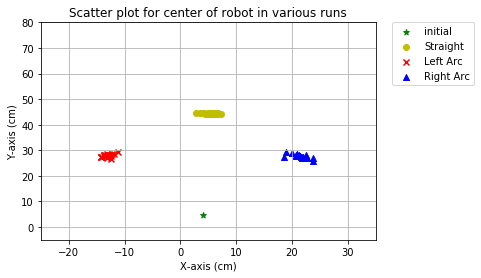
\includegraphics[width=0.9\linewidth]{img/scatter_plot.png}
						 		\caption{Scatter plot for center of robot in various runs}
						 	\end{subfigure}
						 	\caption{Visualizing Robot Position}
					 \end{figure}
					 \begin{figure}[H]
						 	\begin{subfigure}{0.5\textwidth}
						 		\centering
						 		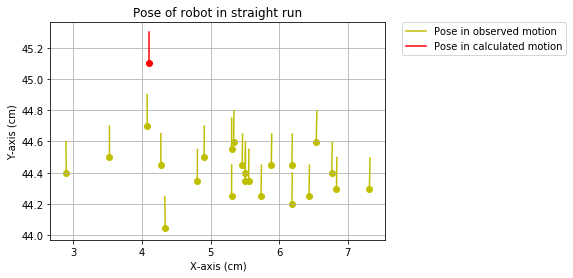
\includegraphics[width=0.8\linewidth]{img/scatter_plot_st.png}
						 		\caption{Pose of robot in Straight run}
						 	\end{subfigure}
						 	\hfill
						 	\begin{subfigure}{0.5\textwidth}
						 		\centering
						 		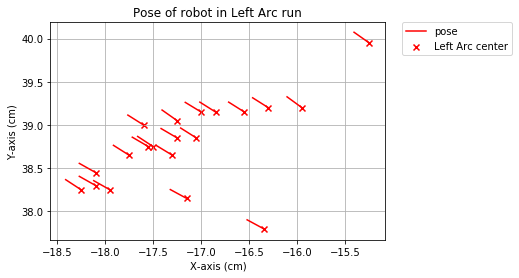
\includegraphics[width=0.8\linewidth]{img/scatter_plot_lt.png}
						 		\caption{Pose of robot in Left Arc run}
						 	\end{subfigure}
						 	\begin{subfigure}{0.5\textwidth}
						 		\centering
						 		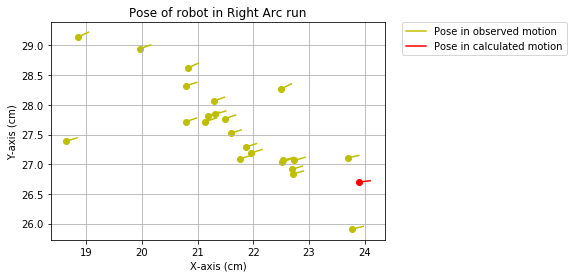
\includegraphics[width=0.8\linewidth]{img/scatter_plot_rt.png}
						 		\caption{Pose of robot in Right Arc run}
						 	\end{subfigure}
						 	\caption{Zoomed View of Robot Positions}
				     \end{figure}	
				All the plots and code is available in the file "SEE\_Experiment03\_calculations.ipynb"\\
				\subsection{\textcolor{blue}{Uncertainty of Measurement}}
				The estimated uncertainty of measurement for position and rotation is $4.5$ millimeters and $0.5^{\circ}$ respectively.  
				\begin{itemize}
					\item The uncertainty for rotation occurs because of taking the readings manually using protractor and sometimes the value falls in between two points and we took nearest round value. Hence the uncertainty of measurement in this case is $0.5^{\circ}$.
					
					\item  The pen used for marking the position was fixed but still there is a small movement of maximum 4 millimeters possible which contributes to the uncertainty of position measurement.
					
					\item Moreover, position measurements sometimes falls between two values in millimeter scale and we took the nearest value. This contributes maximum $0.5$ millimeters of uncertainty of position measurement.
				\end{itemize}
				\subsection{Software and Libraries used}
				\begin{itemize}
					\item \textbf{LibreOffice Calc} for data recording and initial transformation calculations.
					\item \textbf{Python} for data visualization and calculations
					\item Python libraries:
					\begin{itemize}
						\item pandas
						\item numpy
						\item matplotlib
						\item seaborn
						\item scipy.stats
					\end{itemize}
				\end{itemize}		
				
			\section{\textcolor{blue}{Results}}
			\subsection{Final Position \& Accuracy }
			\begin{itemize}
				\item Straight Run:		
					\begin{itemize}
						\item Mean X value: 5.4 cm
						\item Mean Y value: 44.4 cm
						\item Mean Angular value: 89 degrees
						\item Standard Deviation in X value: 1.0 cm
						\item Standard Deviation in Y value: 0.1 cm
						\item Standard Deviation in Angular value: 1 degrees
						\item Accuracy in X-coordinate: 67.26\%
						\item Accuracy in Y-coordinate: 98.43\%
						\item Accuracy in angular: 98.60\%
					\end{itemize}
				\item Left Arc:
					\begin{itemize}
						\item Mean X value: -13.2 cm
						\item Mean Y value: 27.9 cm
						\item Mean Angular value: 166 degrees
						\item Standard Deviation in X value: 0.8 cm
						\item Standard Deviation in Y value: 0.6 cm
						\item Standard Deviation in Angular value: 2 degrees
						\item Accuracy in X-coordinate:  84.85\%						
						\item Accuracy in Y-coordinate:   95.03\%
						\item Accuracy in angular:  89.96\%
					\end{itemize}
				\item Right Arc	:
					\begin{itemize}
						\item Mean X value: 21.6 cm
						\item Mean Y value: 27.6 cm
						\item Mean Angular value: 17 degrees
						\item Standard Deviation in X value: 1.3 cm
						\item Standard Deviation in Y value: 0.7 cm
						\item Standard Deviation in Angular value: 3 degrees
						\item Accuracy in X-coordinate:   90.38\%
						\item Accuracy in Y-coordinate:   96.73\%
						\item Accuracy in angular:  87.22\%
					\end{itemize}	
			\end{itemize}
			The details of calculations of these values is available in the file "SEE\_Experiment03\_calculations.ipynb"
			\subsection{Compare Data with Gaussian}
			To verify if the observed data follows a gaussian distribution, we use a the \textit{scipy} library. The \textit{scipy.stats.normaltest} function is used to check if the data follows a normal distribution. 
			
			We observe that the threshold value of $p$ value is more than $0.05$,indicating that the data is normally distributed.
			
			However, for the right arc motion, we see that the data observed do not follow a Gaussian distribution, this can be attributed to some outlying data points. The reason for these data points has been explored in the expected problems and performance section.
			
			 \begin{figure}[H]
			 	\begin{subfigure}{\textwidth}
			 		\centering
			 		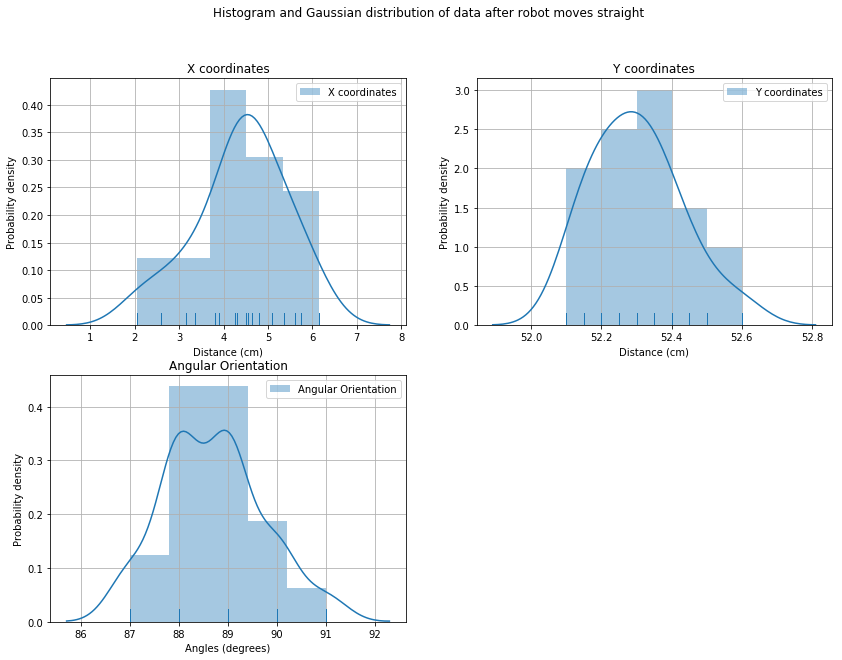
\includegraphics[width=\linewidth]{img/histplot_st.png}
			 		\caption{Histogram and Gaussian distribution of data for straight run}
			 	\end{subfigure}
			 	\caption{}%Histograms and Gaussian distribution of positions along X and Y directions}
			 \end{figure}
			 \begin{figure}[H]
			 	\begin{subfigure}{\textwidth}
			 		\centering
			 		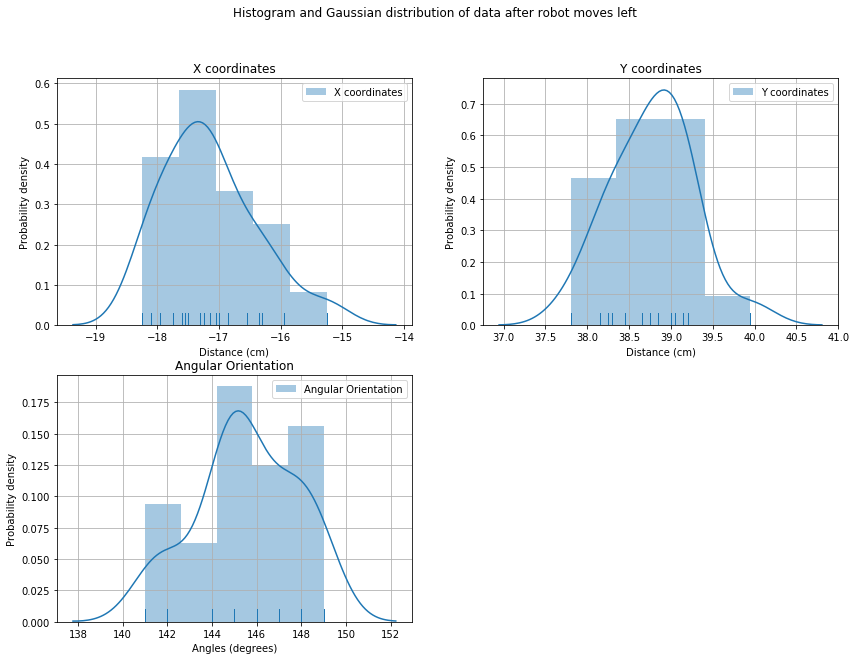
\includegraphics[width=\linewidth]{img/histplot_lt.png}
			 		\caption{Histogram and Gaussian distribution of data for left run}
			 	\end{subfigure}
			 	\caption{}%Histograms and Gaussian distribution of positions along X and Y directions}
			\end{figure}
			\begin{figure}[H]
			 	\begin{subfigure}{\textwidth}
			 		\centering
			 		
\includegraphics[width=\linewidth]{img/histplot_rt.png}
			 		\caption{Histogram and Gaussian distribution of data for right run}
			 	\end{subfigure}
			 	\caption{}%Histograms and Gaussian distribution of positions along X and Y directions}
			 \end{figure}	
			\end{document}
